%%%%%%%%%%%%%%%%
%% Preambule  %%
%%%%%%%%%%%%%%%%

\documentclass[11pt]{article}

\usepackage{amsmath,amsfonts,amssymb}
\usepackage{upgreek}
\usepackage{enumerate}
\usepackage{enumitem}   %
\usepackage{multicol}
\usepackage{scrextend}
\usepackage{fancyhdr}
\usepackage{lastpage}
\usepackage{subcaption} % 2 column images
\usepackage[all]{xy}
\usepackage{tikz-qtree}
\usepackage[margin=2.5cm]{geometry}
\input{../../Template/fitch.sty}

\setlength{\parindent}{0pt}

\pagestyle{fancy}

\lhead{\opdrachtNaam\ \opdrachtNummer}
\rhead{\naam(\studentNummer)}
\rfoot{Pagina\ \thepage\ van\ \pageref{LastPage}}
\lfoot{\datum}
\cfoot{}

\renewcommand\headrulewidth{0.4pt}
\renewcommand\footrulewidth{0.4pt}

\newcommand{\E}{\exists}
\newcommand{\A}{\forall}

\newcommand{\ccen}[2]{\llap{$#1$}${}\mathrel{\circ}{}$\rlap{$#2$}}

%%%%%%%%%%%%%%
%% Gegevens %%
%%%%%%%%%%%%%%

\newcommand{\naam}          {Stefan Schenk}
\newcommand{\studentNummer} {11881798}
\newcommand{\opdrachtNaam}  {Assignment}
\newcommand{\opdrachtNummer}{3}
\newcommand{\datum}         {November 2017}

%%%%%%%%%%%%%%%%
%% Antwoorden %%
%%%%%%%%%%%%%%%%

\begin{document}

% Opgaven:
%
% The exercises for Homework 3 are:
%  5.31(g), 5.32(2,3), 5.33(2), 5.37(2,3, van rechts naar links), 5.38(3), 5.53(Quine dolk)

\subsection*{Opgave 5.31}

%  Hint for exercise 5.31(g): For the last step of the proof, you need to use the rule G V (gebruik rule for the disjunction) with phi_1 = q and phi_2 = r and psi is the formula (p ∧ q) ∨ (p ∧ r).

(g) $p\wedge(q\vee r) \vdash (p\wedge q)\vee(p\wedge r)$

\[
\begin{nd}
 \hypo {1} {p\wedge(q\vee r) \vdash (p\wedge q)\vee(p\wedge r)}
 \open
 \hypo {2} {\exists x P(x)}
 \open[u]
 \hypo {3} {P(u)}
 \have {4} {\forall y \neg P(y)}  \r{1}
 \have {5} {\neg P(u)}            \Ae{4}
 \have {6} {\bot}                 \ne{3,5}
 \close
 \have {6a}{\bot}                 \Ee{2,3-6}
 \close
 \have {7} {\neg \exists x P(x)}  \ni{2-6a}
\end{nd}
\]

\subsection*{Opgave 5.32}

(2) $p\wedge (q\wedge r) \vdash r \wedge p$

(3) $p \rightarrow (q\wedge r), q \rightarrow s, p\vdash s$

\subsection*{Opgave 5.33}

(2) $\varphi\vee(\psi\wedge\chi);
  (\varphi\vee\psi)\wedge(\varphi\vee\chi)$

\begin{center}
  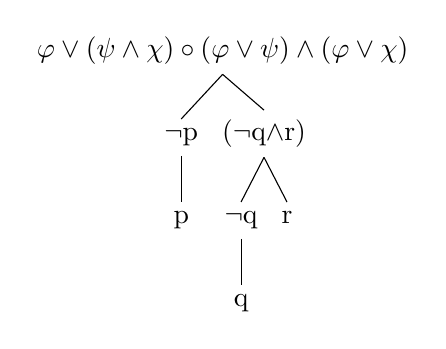
\begin{tikzpicture}
    \Tree [.$\varphi\vee(\psi\wedge\chi)\circ(\varphi\vee\psi)\wedge    (\varphi\vee\chi)$ [.$\neg$p [.p ] ]
    [.($\neg$q$\wedge$r) [.$\neg$q q ]
    [.r ]]]
  \end{tikzpicture}
\end{center}

\subsection*{Opgave 5.37}

(2) $\varphi\leftrightarrow\psi;
  (\varphi\rightarrow\psi)\wedge(\psi\rightarrow\varphi)$

\begin{center}
  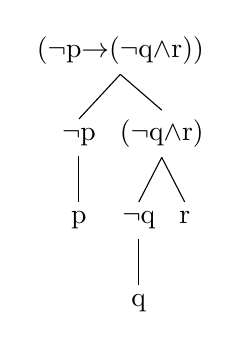
\begin{tikzpicture}
    \Tree [.($\neg$p$\rightarrow$($\neg$q$\wedge$r)) [.$\neg$p [.p ] ]
    [.($\neg$q$\wedge$r) [.$\neg$q q ]
    [.r ]]]
  \end{tikzpicture}
\end{center}

(3) $\varphi\rightarrow\psi;
  \neg\psi\rightarrow\neg\varphi$

\begin{center}
  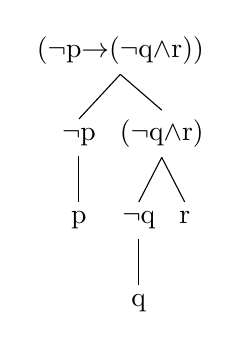
\begin{tikzpicture}
    \Tree [.($\neg$p$\rightarrow$($\neg$q$\wedge$r)) [.$\neg$p [.p ] ]
    [.($\neg$q$\wedge$r) [.$\neg$q q ]
    [.r ]]]
  \end{tikzpicture}
\end{center}

\subsection*{Opgave 5.38}

(3) $((p\rightarrow q)\wedge(q\rightarrow r))\rightarrow(p\rightarrow r)$

\begin{center}
  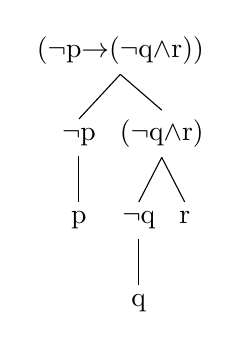
\begin{tikzpicture}
    \Tree [.($\neg$p$\rightarrow$($\neg$q$\wedge$r)) [.$\neg$p [.p ] ]
    [.($\neg$q$\wedge$r) [.$\neg$q q ]
    [.r ]]]
  \end{tikzpicture}
\end{center}

\subsection*{Opgave 5.53}

\textit{Geef de semantische tableauregels voor de Quine dolk $\dagger$.}



%  5.31(g), 5.32(2,3), 5.33(2), 5.37(2,3, van rechts naar links), 5.38(3), 5.53(Quine dolk)%%%%%%%%%%%%%%%%%%%%

\end{document}
